\chapter{Modelización de las redes neuronales} \label{ch:modelizacion}

A partir de las herramientas matemáticas que hemos introducido en \customref{ch:matematicas_fundamentales} y de la modelización de la tarea de aprendizaje realizada en \customref{ch:tarea_aprendizaje}, buscamos desarrollar una modelización matemática de las redes neuronales con las que se suele trabajar en la práctica. Para que sea una \textbf{buena modelización}, esta debería cumplir que:

\begin{itemize}
    \item Sea lo más parecida a los modelos que se usan en la práctica
    \item Permita obtener resultados interesantes
\end{itemize}

Usando descomposiciones tensoriales, modelaremos dos tipos de redes:

\begin{itemize}
    \item Redes neuronales no profundas, a partir
    \todo{no se que nombre le dan a cada una de las redes en el paper!}
    \item Redes convolucionales profundas, a partir de los \textit{circuitos convolucionales aritméticos}
\end{itemize}

Creemos que la \textbf{modelización es muy cercana a las redes usadas en la práctica}. Principalmente, porque tiene en cuenta las tres propiedades características de una red convolucional:

\begin{enumerate}
    \item Localidad
    \item Compartición de parámetros, que junto a la localidad, da lugar a la convolución
    \item \textit{Pooling}
\end{enumerate}
\todo{Esto ya lo digo antes en la introducción. No sé si aquí sería buen momento para desarrollar lo que significa cada cosa o si es mejor quitarlo de alguna parte}

Además, los \textit{circuitos convolucionales aritméticos} son equivalentes a las redes conocidas como \textit{SimNets}, lo que reafirma el hecho de que la modelización es muy buena.
\todo{Esta afirmación la tendría que justificar, aunque sea referenciando al paper principal}

\section{Modelo CP}

Como ya hemos comentado en \customref{sec:repr_funciones_puntuacion}, buscaremos descomponer el tensor de coeficientes $\mathcal{A}^y$ que aparece en la ecuación \eqref{eq:puntuacion_general}, para que el aprendizaje de sus coeficientes sea computacionalmente factible.

La idea más simple es aplicar la \textit{descomposición CP}, que introducimos en \eqref{eq:cp_decomp}, en la ecuación \eqref{eq:puntuacion_general}. Usaremos una descomposición conjunta para los tensores:

\begin{equation} \label{eq:cp_decomp_conjunta}
    \mathcal{A}^y = \sum_{z = 1}^Z a_z^y \cdot \nv{\omega^{z, 1}} \otimes \ldots \otimes \nv{\omega^{z, N}}
\end{equation}

\todo{En la ecuación que introduzco antes no tengo escalares en la sumatoria!}

Desarrollemos los elementos que participan en esa ecuación. En primer lugar, sabemos por \eqref{eq:cp_decomp} que $a_z^y \in \R$, y por tanto, podemos considerar $\nv{a^y} := (a_1^y, \ldots, a_Z^y)^T \in \R^Z$. En segundo lugar, y de nuevo, conforme a \eqref{eq:cp_decomp}, tenemos los vectores $\nv{\omega^{z, i}} \in \R^M$ con $z \in \deltaset{Z}$, $i \in \deltaset{N}$. Decimos que la \textbf{descomposición es conjunta} porque los vectores $\nv{\omega^{z, i}}$ son los mismos para todos los valores de $y \in \mathcal{Y}$. Solo cambian los coeficientes $\nv{a^y}$, como bien refleja la elección de índices de la fórmula.

\begin{proposicion}
    Tomando $Z = M^N$ en la ecuación \refeq{eq:cp_decomp_conjunta}, la descomposición es universal. Esto es, podemos fijar un conjunto de vectores $\{\nv{\omega^{z, i}} \in \R^M / z \in \deltaset{Z}, i \in \deltaset{N} \}$ de forma que cualquier tensor $\mathcal{A}^y$ de orden $N$ y dimensión $M$ en cada modo puede ser representado. Es decir:

    \begin{equation}
        \forall \mathcal{A}^y \in \espaciotensores{N}{M}, \exists \nv{a^y} \in \R^Z: \text{la ecuación \refeq{eq:cp_decomp_conjunta} se verifica}
    \end{equation}
\end{proposicion}

\begin{proof}
    La idea de la demostración es muy sencilla. Tenemos que expresar un tensor arbitrario $\mathcal{A}$ de orden $N$ y dimensión $M$ en cada modo (es decir, de $M^N$ elementos) como una suma de $M^N$ elementos. Por tanto, en cada sumando, buscamos generar un único elemento del tensor y colocarlo en los índices apropiados. Es decir, cada sumando será un tensor de todo ceros salvo la entrada de la que nos ocupamos en esa iteración.

    Para que la demostración sea más clara cambiaremos la forma de indexar la suma. En la proposición estamos usando un único índice que llega hasta $Z = M^N$. Esto es lo mismo que usar $N$ índices que lleguen hasta $M$, y así la sumatoria queda:

    \begin{equation}
        \mathcal{A} = \sum_{i_1 = 1, \ldots, i_N = 1}^M a_{(i_1, \ldots, i_N)} \cdot \nv{\omega^{(i_1, \ldots, i_N), 1}} \otimes \ldots \otimes \nv{\omega^{(i_1, \ldots, i_N), N}}
    \end{equation}

    Para llevar a cabo la idea de usar cada sumando para colocar un elemento de $\mathcal{A}$ en sus índices correctos, haremos que en cada sumando se verifique

    \begin{itemize}
        \item $a_{i_1, \ldots, i_N} = \mathcal{A}_{i_1, \ldots, i_N}$. Esto es inmediato y no necesita más explicación
        \item $\nv{\omega^{(i_1, \ldots, i_N), 1}} \otimes \ldots \otimes \nv{\omega^{(i_1, \ldots, i_N), N}}$ genere el tensor en $\espaciotensores{N}{M}$ que sea cero en todas las entradas salvo en el índice $(i_1, \ldots, i_N)$, donde valdrá 1. Dicho tensor lo podemos denotar como  $\mathcal{B}^{(i_1, \ldots, i_N)}$
    \end{itemize}

    Ahora, veamos cómo podemos generar el tensor $\mathcal{B}^{(i_1, \ldots, i_N)}$ como producto tensorial de ciertos vectores. La propiedad fundamental que queremos que ese tensor cumpla es:

    \begin{equation}
        \mathcal{B}^{(i_1, \ldots, i_N)}_{j_1, \ldots, j_N} =
        \begin{cases}
            1 & \text{si } i_1 = j_1, \ldots, i_N = j_N \\
            0 & \text{en otro caso}
        \end{cases}
    \end{equation}

    Definimos $\nv{\delta_{i, N}}$ como el vector de longitud $N$, con todas las entradas nulas salvo la entrada de la posición $i$, en la que ponemos un uno. Por tanto, es claro que:

    \begin{equation}
        (\nv{\delta_{i, N}})_k =  \delta_{i, k}
    \end{equation}

    Definimos

    \begin{equation}
        \mathcal{B}^{(i_1, \ldots, i_N)} := \nv{\delta_{i_1, N}} \otimes \ldots \otimes \nv{\delta_{i_N, N}}
    \end{equation}

    y por tanto se verifica que:

    \begin{equation}
        \mathcal{B}^{(i_1, \ldots, i_N)}_{j_1, \ldots, j_N} = (\vec{\delta}_{i_1, N})_{j_1} \cdot \ldots \cdot (\vec{\delta}_{i_N, N})_{j_N} = \delta_{i_1, j_1} \cdot \ldots \cdot \delta_{i_N, j_N} =
        \begin{cases}
            1 & \text{si } i_1 = j_1, \ldots, i_N = j_N \\
            0 & \text{en otro caso}
        \end{cases}
    \end{equation}

    como buscábamos. Para concluir la demostración, fijamos el conjunto de vectores de forma que:

    \begin{equation} \label{eq:cp_decomp_asignacion_vectores}
        \{\nv{\omega^{z, i}} \in \R^M / z \in \deltaset{Z}, i \in \deltaset{N} \} =
        \{ \nv{\delta_{i_j, N}} / j \in \deltaset{N}, i_j \in \deltaset{M} \}
    \end{equation}

\end{proof}

\begin{observacion}
    En \eqref{eq:cp_decomp_asignacion_vectores} vemos que estamos usando menos vectores que los que se consideran en el enunciado del teorema. Esto es porque estamos repitiendo estos vectores. Por ejemplo, todos los sumandos referentes al valor 1 del primer índice tiene como primer vector $\vec{\delta}_{1, N}$
\end{observacion}

\begin{observacion}
    Esta proposición nos sirve para tener una cota superior del número de sumandos necesarios para realizar la descomposición. No hemos ganado nada respecto al trabajo previo. Seguimos teniendo el problema de considerar $M^N$ elementos, problema que ya vimos en \customref{sec:justificacion_func_repr}
\end{observacion}

Veamos ahora cómo podemos aplicar esta descomposición conjunta en nuestra ecuación \customref{eq:puntuacion_general}. Partimos de las dos ecuaciones:

\begin{equation}
\begin{split}
    h_y(\nv{x_1}, \ldots, \nv{x_N}) &= \sum_{d_1, \ldots, d_N = 1}^{M} \mathcal{A}^y_{d_1, \ldots, d_N} \prod_{i = 1}^N f_{\theta_{d_i}}(\nv{x_i}) \\
    \mathcal{A}^y &= \sum_{z = 1}^Z a_z^y \cdot \nv{\omega^{z, 1}} \otimes \ldots \otimes \nv{\omega^{z, N}} \\
\end{split}
\end{equation}

Ahora, sustituimos la segunda ecuación en la primera:

\begin{equation}
\begin{split}
    h_y(\nv{x_1}, \ldots, \nv{x_N}) &= \sum_{d_1, \ldots, d_N = 1}^{M} (\sum_{z = 1}^Z a_z^y \cdot \nv{\omega^{z, 1}} \otimes \ldots \otimes \nv{\omega^{z, N}}) \prod_{i = 1}^N f_{\theta_{d_i}}(\nv{x_i}) = \ldots \\
    \ldots &=  \sum_{z = 1}^Z \dspace \sum_{d_1, \ldots, d_N = 1}^{M} a_z^y \cdot \nv{\omega^{z, 1}} \otimes \ldots \otimes \nv{\omega^{z, N}} \prod_{i = 1}^N f_{\theta_{d_i}}(\nv{x_i}) = \ldots \\
    \ldots &=  \sum_{z = 1}^Z a_z^y \sum_{d_1, \ldots, d_N = 1}^{M} \nv{\omega^{z, 1}} \otimes \ldots \otimes \nv{\omega^{z, N}} \prod_{i = 1}^N f_{\theta_{d_i}}(\nv{x_i}) = \ldots \\
    \ldots &=  \sum_{z = 1}^Z a_z^y \sum_{d_1, \ldots, d_N = 1}^{M} \dspace \prod_{i = 1}^N \nv{\omega^{z, 1}} \otimes \ldots \otimes \nv{\omega^{z, N}} \cdot f_{\theta_{d_i}}(\nv{x_i}) = \ldots \\
    \ldots &=  \sum_{z = 1}^Z a_z^y \dspace \prod_{i = 1}^N \dspace \sum_{d_1, \ldots, d_N = 1}^{M}  \nv{\omega^{z, 1}} \otimes \ldots \otimes \nv{\omega^{z, N}} \cdot f_{\theta_{d_i}}(\nv{x_i}) = \ldots \\
    \ldots &=  \sum_{z = 1}^Z a_z^y \dspace \prod_{i = 1}^N \dspace \sum_{d = 1}^{M} \omega^{z, i}_d \cdot f_{\theta_{d}}(\nv{x_i})
\end{split}
\end{equation}
\todo{Tengo que desarrollar en papel bien este desarrollo que no tengo nada claro. El último paso no lo tengo controlado. Es la eq. (3) del paper de referencia}

Por lo tanto, nuestro \textbf{Modelo CP} se puede describir con la ecuación:

\begin{equation} \label{eq:cp_model}
    h_y(\nv{x_1}, \ldots, \nv{x_N}) =  \sum_{z = 1}^Z a_z^y \dspace \prod_{i = 1}^N \dspace \sum_{d = 1}^{M} \omega^{z, i}_d \cdot f_{\theta_{d}}(\nv{x_i})
\end{equation}

\subsection{Desarrollo del modelo}
\todo{Mejor nombre para esta sección}

Veamos cómo esta ecuación se relaciona con un modelo usual de \textit{machine learning}. En primer lugar, y como ya hemos comentado en \customref{sec:repr_funciones_puntuacion}, el primer paso de nuestro modelo puede considerarse computar la capa de representación, esto es, los valores

$$\{f_{\theta_d}(\nv{x_i}) / d \in \deltaset{M},\ i \in \deltaset{N} \}$$

Una vez hecho esto, en \eqref{eq:cp_model} podemos ver $\sum_{d = 1}^{M} \omega^{z, i}_d \cdot f_{\theta_{d}}(\nv{x_i})$ como un bloque convolucional sobre los $d$ elementos de la capa de representación que estamos considerando para el índice $i$. Por tanto, podríamos pensar ahora mismo en la ecuación como:

\begin{equation}
    h_y(\nv{x_1}, \ldots, \nv{x_N}) =  \sum_{z = 1}^Z a_z^y \dspace \prod_{i = 1}^N \dspace Conv(i)
\end{equation}

Dicha convolución puede variar sus coeficientes dependiendo de la localización en la que nos encontremos sobre la capa de representación. Esto no es lo usual en la práctica, así que en \customref{subs:comparticion_parametros_cp} resolvemos este problema. Y escrita la ecuación de esta forma, es claro que estamos generando $N$ \textit{feature maps} para un valor de $z$ determinado.

Escrito así, también es claro que el productorio está actuando como un \textit{pooling} sobre los ya mencionados $N$ \textit{feature maps}. Es un \textit{pooling} de tipo producto que nos devuelve un escalar. De nuevo, re-escribimos la ecuación:

\begin{equation}
    h_y(\nv{x_1}, \ldots, \nv{x_N}) =  \sum_{z = 1}^Z a_z^y \dspace ProdPooling( Conv(i) )
\end{equation}

Y con esto, vemos que la sumatoria final está combinando los escalares producidos por la convolución seguida del \textit{pooling} de forma lineal. Esto es, una \textit{linear dense layer} sobre dichos $Z$ escalares.

En resumen, tras computar la capa de representación, nuestro modelo tiene una capa oculta sobre la que aplicamos \textit{pooling}, que combinamos en una capa densa. Y por tanto, es razonable considerar este modelo con lo que se conoce comúnmente como una \textbf{red \textit{shallow}}.

Podemos representar este modelo gráficamente como sigue:

\begin{figure}[h]
\centering
\begin{tikzpicture}[
    squarenode/.style={rectangle, draw=cyan!60, fill=cyan!5, very thick, minimum size=5mm, align=center},
]
    \node [squarenode] (entrada) {\textbf{Datos de entrada}\\ \\ $X = (\nv{x_1}, \ldots, \nv{x_N})$};
    \node [squarenode]  (repr) [right=2.0cm of entrada] {\textbf{Capa de representación}\\ \\ $f_{\theta_d}(\nv{x_i})$};
    \node [squarenode] (convoluciones) [below=2.0cm of repr] {\textbf{\textit{Feature maps}}\\ \\ $\sum_{d = 1}^{M} \omega^{z, i}_d \cdot f_{\theta_{d}}(\nv{x_i})$};
    \node [squarenode] (pooling) [left=2.0cm of convoluciones] {\textbf{$Z$ Escalares tras el pooling}\\ \\ $\prod_{i = 1}^N \dspace \sum_{d = 1}^{M} \omega^{z, i}_d \cdot f_{\theta_{d}}(\nv{x_i})$};
    \node [squarenode] (denselayer) [below=2.0cm of pooling] {\textbf{Puntuación para la etiqueta $y$} \\ \\$h_y(\nv{x_1}, \ldots, \nv{x_N})$};

    \draw[-stealth] (entrada.east) -- node[text width=2.0cm,midway,above,align=center]{$f_d$} (repr.west);
    \draw[-stealth] (repr.south) -- node[text width=2.0cm,midway,right,align=center]{Convoluciones $\sum_{d = 1}^{M} \omega^{z, i}_d \cdot $} (convoluciones.north);
    \draw[-stealth] (convoluciones.west) -- node[text width=2.0cm,midway,above,align=center]{Pooling $\prod_{i = 1}^N$} (pooling.east);
    \draw[-stealth] (pooling.south) -- node[text width=2.0cm,midway,right,align=center]{Dense layer $\sum_{z = 1}^Z a_z^y$} (denselayer.north);

\end{tikzpicture}
\caption{Representación gráfica del modelo \textit{CP}}
\end{figure}

\subsection{Compartición de parámetros} \label{subs:comparticion_parametros_cp}

Ya hemos comentado previamente que las convoluciones pueden variar sus coeficientes dependiendo de la localización. Lo usual en la práctica es usar los mismos coeficientes independientemente de la localización, lo que se conoce como \textbf{compartición de parámetros}.

La compartición de coeficientes es necesaria para que identificar ciertos patrones en la imagen no dependa de la localización del patrón en la imagen. Por ejemplo, una cara debería detectarse como tal independientemente de la localización de esta.

En el modelo \textit{CP}, la variación de los coeficientes dependiendo de la localización viene dada por la dependencia en $i$ de $\sum_{d = 1}^M \omega_d^{z ,i}$.

Por tanto, para forzar el deseado \textit{coefficient sharing} basta con imponer en \eqref{eq:cp_decomp_conjunta}:

\begin{equation}
    \nv{w^{z, 1}} = \ldots = \nv{w^{z, N}} =: \nv{w^z}
\end{equation}

Esto convierte la descomposición \textit{CP} en una descomposición \textit{CP} simétrica, es decir:

\begin{equation}
    \mathcal{A}^y = \sum_{z = 1}^Z a_z^y \cdot \comentardebajo{\nv{a^z} \otimes \ldots \otimes \nv{a^z}}{N veces}; \dspace \nv{a^z} \in \R^M
\end{equation}

Por lo tanto, \textbf{perdemos la universalidad del modelo}: no podemos representar cualquier tensor, independientemente de lo grande que sea $Z$. Solo podemos representar tensores simétricos.

\subsection{Parámetros del modelo} \label{msubsec:parametros_modelo_cp}

A partir de la ecuación \eqref{eq:cp_model} vemos que para definir nuestro modelo debemos definir los coeficientes:

\begin{itemize}
    \item $\{a_z^y \in \R : z \in \deltaset{Z}, \dspace y \in \deltaset{Y}\}$, lo que supone $Y \cdot Z$ coeficientes
    \item $\{\omega_d^{z, i} \in \R: i \in \deltaset{N}, \dspace z \in \deltaset{Z}, \dspace d \in \deltaset{M}\}$, lo que lo que supone $N \cdot M \cdot Z$ coeficientes
\end{itemize}

Es decir, que en total nuestro modelo viene dado al especificar $N \cdot M \cdot Z + Y \cdot Z$ coeficientes.

\section{Modelo HT} \label{sec:modelo_ht}

En esta sección pasamos a presentar el segundo y último modelo con el que trabajaremos. A diferencia del modelo anterior, esta vez terminaremos con una arquitectura que puede considerarse como profunda. La idea principal consiste en expresar el tensor de coeficientes $\mathcal{A}^y$ con su descomposición jerárquica de \textit{Tucker}, o como se la conoce por sus siglas en inglés, \textbf{descomposición \textit{HT}} \footnote{Dicha descomposición se introduce en \cite{matematicas:descomposicion_ht}. Nosotros usaremos una versión concreta, introducida por \cite{matematicas:principal}, restringiendo las matrices de \cite{matematicas:descomposicion_ht}}.

Desarrollamos ahora el tensor $\mathcal{A}^y$ recursivamente, de la siguiente forma:

\begin{equation} \label{eq:descomposicion_ht}
\begin{split}
    \phi^{1, j, \gamma} &:= \sum_{\alpha = 1}^{r_0} a_{\alpha}^{1, j, \gamma} \cdot \nv{\varphi^{2j-1, \alpha}} \otimes \nv{\varphi^{2j, \alpha}} \\
    \ldots \\
    \phi^{l, j, \gamma} &:= \sum_{\alpha = 1}^{r_{l-1}} a_{\alpha}^{l, j, \gamma} \cdot \phi^{l-1, 2j-1, \alpha} \otimes \phi^{l-1, 2j, \alpha} \\
    \ldots \\
    \phi^{L - 1, j, \gamma} &:= \sum_{\alpha = 1}^{r_{L-2}} a_{\alpha}^{L - 1, j, \gamma} \cdot \phi^{L-2, 2j-1, \alpha} \otimes \phi^{L-2, 2j, \alpha} \\
    \mathcal{A}^y &:= \sum_{\alpha = 1}^{r_{L-1}} a_{\alpha}^{L, y} \cdot \phi^{L-1, 1, \alpha} \otimes \phi^{L-1, 2, \alpha}
\end{split}
\end{equation}

Estudiemos detenidamente la ecuación \eqref{eq:descomposicion_ht}. Para facilitar el entendimiento al lector, hay que tener en cuenta que

\begin{itemize}
    \item El superíndice $l$ indica en que nivel de la descomposición nos encontramos. Consideraremos que en total tenemos $L$ capas
    \item El superíndice $j$ indica la posición en la que nos encontramos dentro del nivel $l$
    \item El superíndice $\gamma$ indica con qué tensor de la capa $l$ y posición $j$ estamos trabajando. Es decir, dados un nivel y una posición, podemos tener más de un tensor
    \item Los valores $r_l$, que llamaremos \textbf{rango de nivel $l$}, marcan el número de tensores que hay en cada posición $j$ de la capa $l$. Considerando que en la primera ecuación no trabajamos con tensores sino con vectores
\end{itemize}

En primer lugar, estamos construyendo el tensor de coeficientes $\mathcal{A}^y$ de forma claramente recursiva. Empezamos construyendo los tensores $\phi^{1, j, \gamma}$ a partir de unos vectores iniciales $\{\nv{\varphi^{j, \alpha}} \in \R^M: j \in \deltaset{N}, \alpha \in \deltaset{r_0}  \}$  y unos coeficientes reales $\{a_{\alpha}^{1, j, \gamma}: \alpha \in \deltaset{r_0}\}$. Los tensores del nivel $l$ se construyen en función de los tensores del nivel $l-1$.

A partir de las fórmulas es claro ver que los tensores de una capa tienen un orden el doble que los de la capa anterior. Esto porque estamos considerando, en las sumatorias, el producto tensorial de dos tensores del mismo orden, y por tanto, su orden se duplica. En el primer paso trabajamos con vectores, que podemos considerar tensores de orden $1$. Por tanto, en una capa $l$ generada por:

\begin{equation}
    \phi^{l, j, \gamma} = \sum_{\alpha = 1}^{r_{l-1}} a_{\alpha}^{l, j, \gamma} \cdot \phi^{l-1, 2j-1, \alpha} \otimes \phi^{l-1, 2j, \alpha}
\end{equation}

estamos operando con tensores $\phi^{l-1, j, \alpha}$ de orden $2^{l-1}$, para obtener el tensor $\phi^{l, j, \gamma}$ de orden $2^l$.

Siguiendo el mismo razonamiento, los tensores $\phi^{L-1; j = 1, 2; \alpha}$ deberán tener un orden la mitad que nuestro tensor de coeficientes $\mathcal{A}^y$, es decir, $N / 2$. Por este motivo y por simplicidad del desarrollo posterior, consideraremos que $N$ (el orden del tensor $\mathcal{A}^y$) es una potencia de dos. Y con ello tenemos que $L := log_2(N)$. Esta asunción también se realiza en \cite{matematicas:descomposicion_ht} y no supone ningún problema.

Cabe destacar también que estamos considerando solo productos tensoriales de dos elementos. Además, estamos combinando únicamente tensores contiguos de cada capa.

El siguiente diagrama muestra el proceso de generación de los tensores, que deja claro todo lo que acabamos de comentar. Por simplicidad, suponemos que $r = 1$. Es decir, que en cada localización $j$ solo tenemos un tensor, independientemente del nivel $l$ en el que nos encontremos.

\begin{figure}[H]
    \centering
    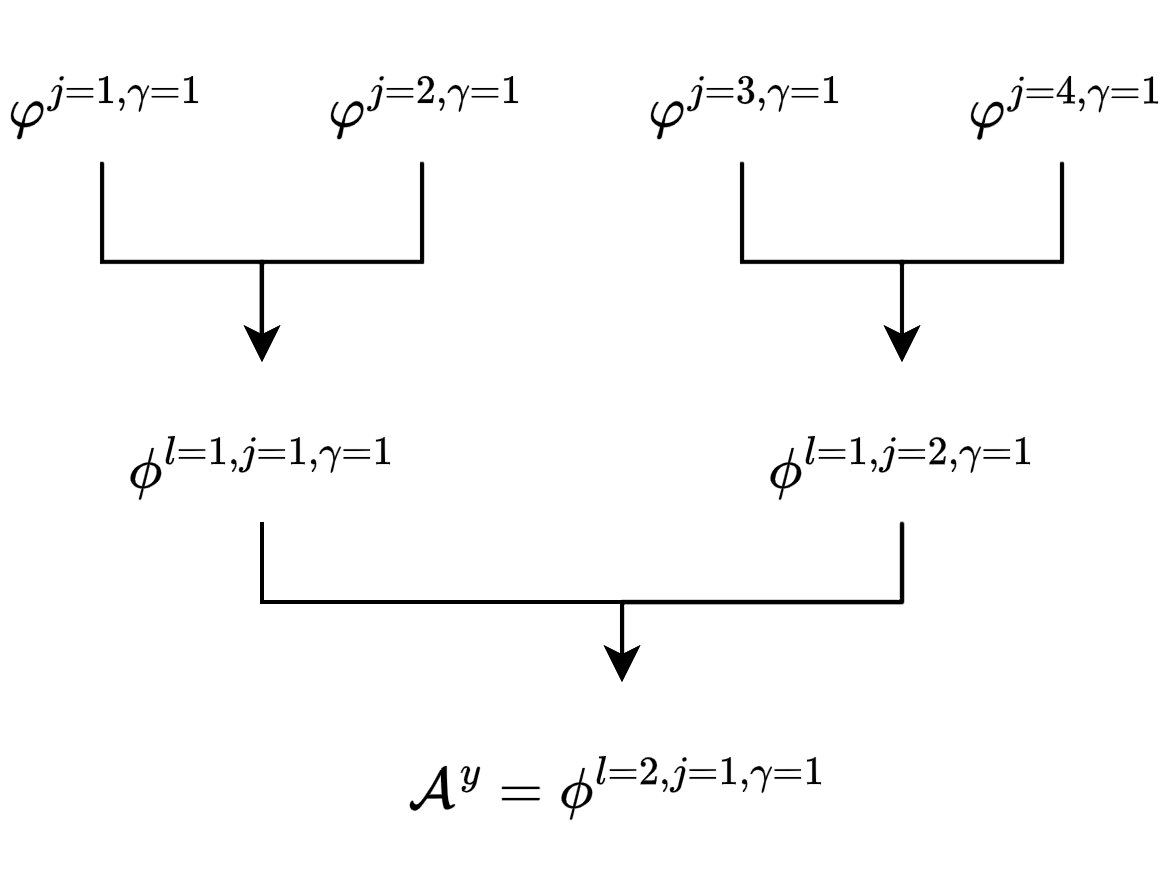
\includegraphics[width=0.6\textwidth]{matematicas/descomp_ht_rank_1}
    \caption{Ejemplo gráfico del proceso de construcción del tensor $\mathcal{A}^y$ a través de la descomposición \textit{HT}. Por simplicidad, estamos suponiendo que $r = 1$. Tenemos $L = 2$ capas o niveles}
    \label{img:diagrama_ht_simple}
\end{figure}

Veamos ahora este mismo diagrama, pero suponiendo que $r = 2$. Por tanto, en cada posición de cada nivel, tendremos dos tensores en vez de uno.

\begin{figure}[H]
\centering
    \ajustarsubcaptions
    \begin{subfigure}{.5\textwidth}
        \centering
        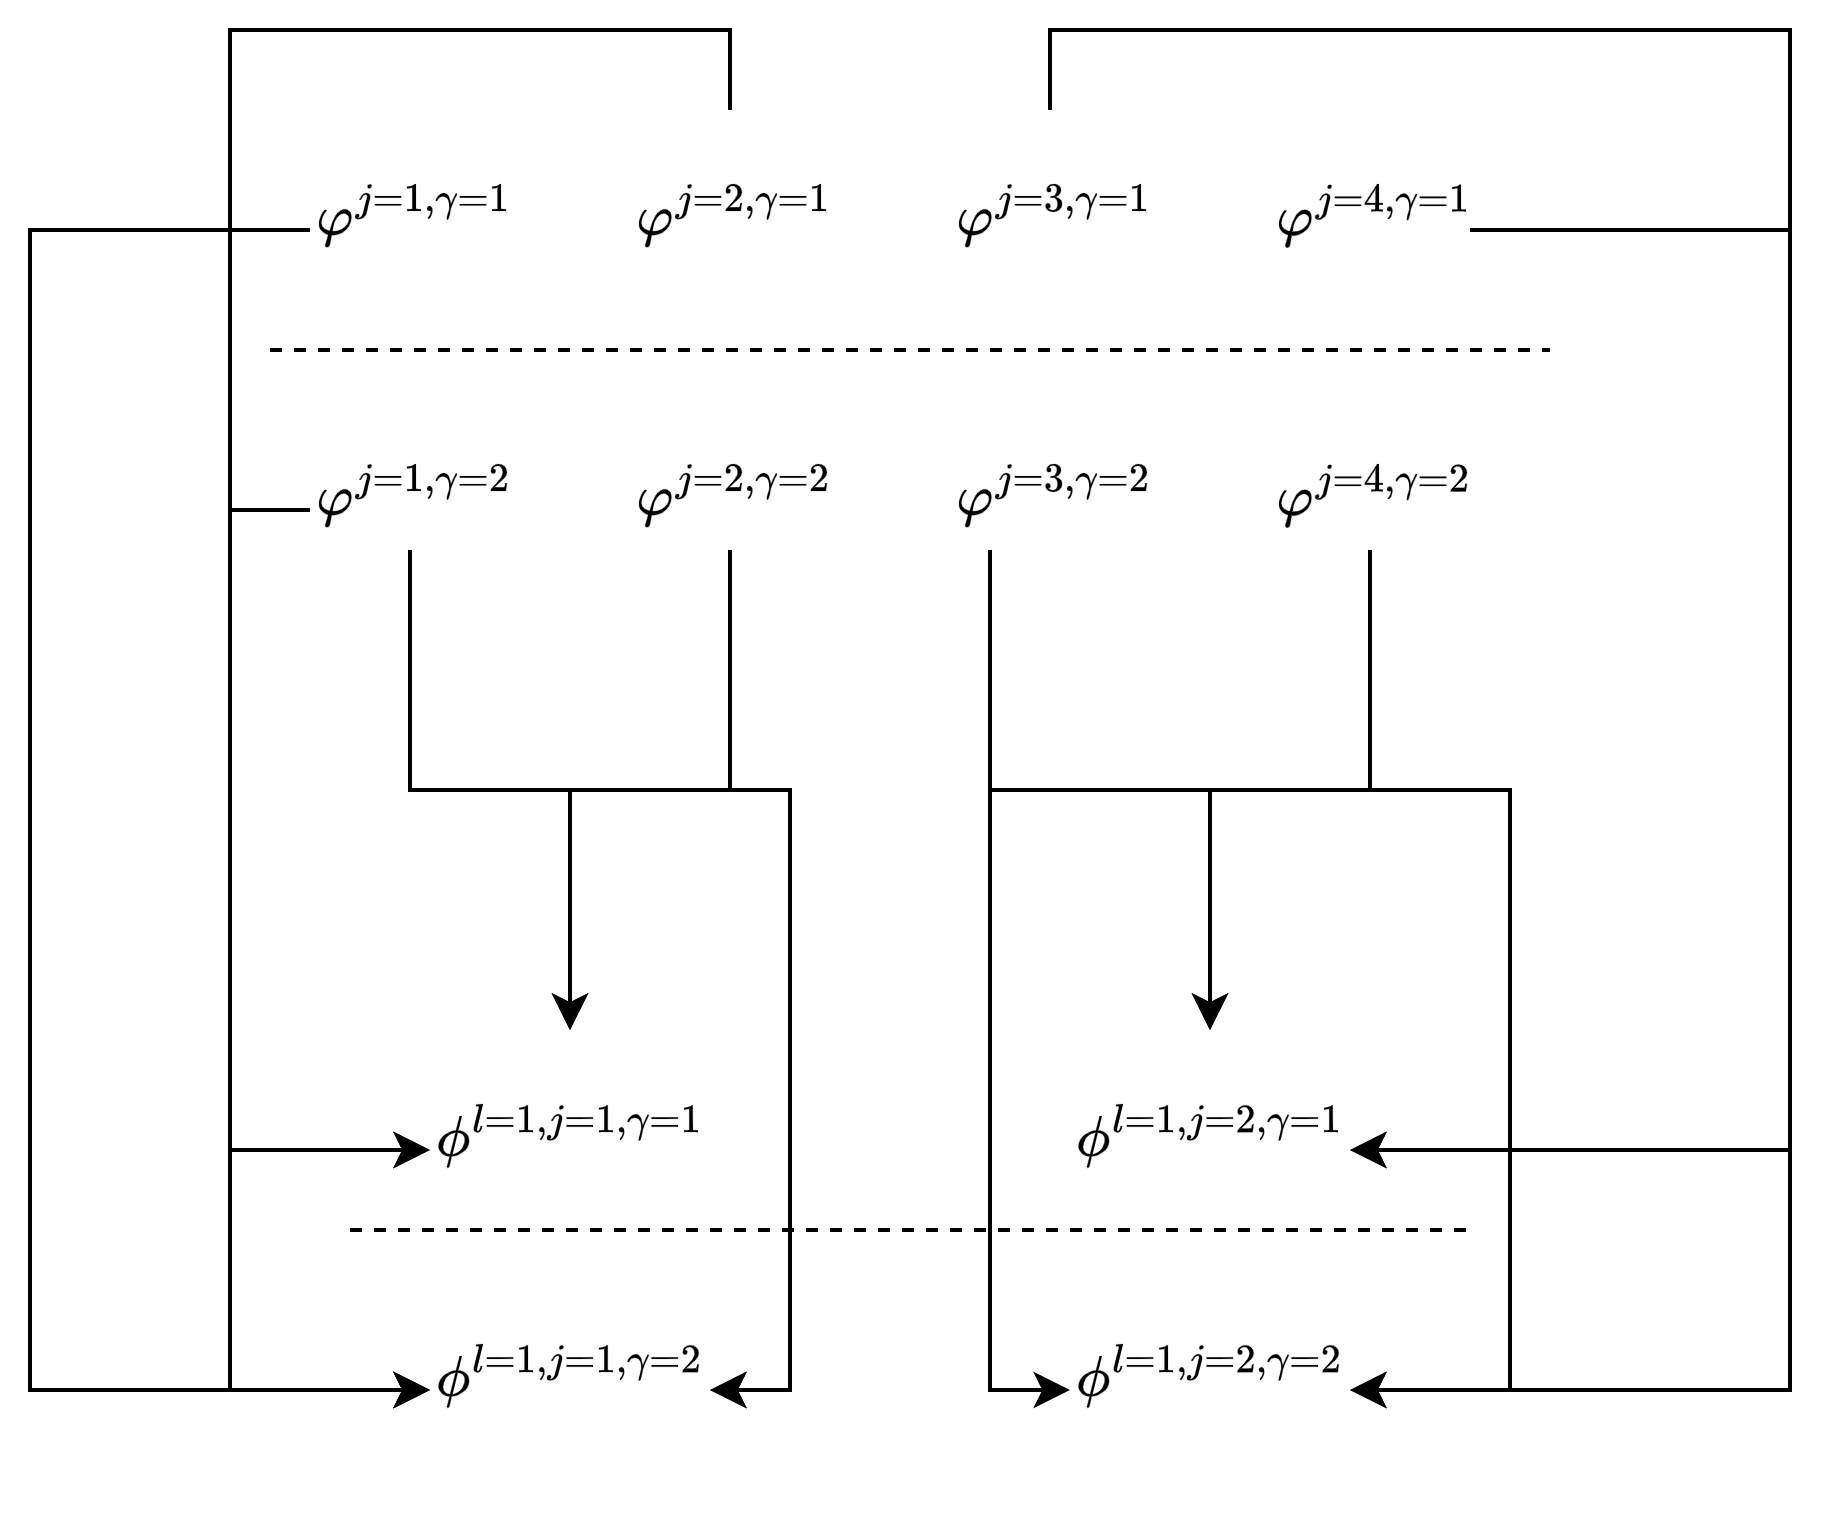
\includegraphics[width=0.9\linewidth]{matematicas/descomp_ht_rank_2_paso_1}
        \caption{Primer paso. En la construcción de cada tensor $\phi^{l, j, \gamma}$ participan cuatro tensores $\varphi^{j, \gamma}$}
    \end{subfigure}%
    \begin{subfigure}{.5\textwidth}
        \centering
        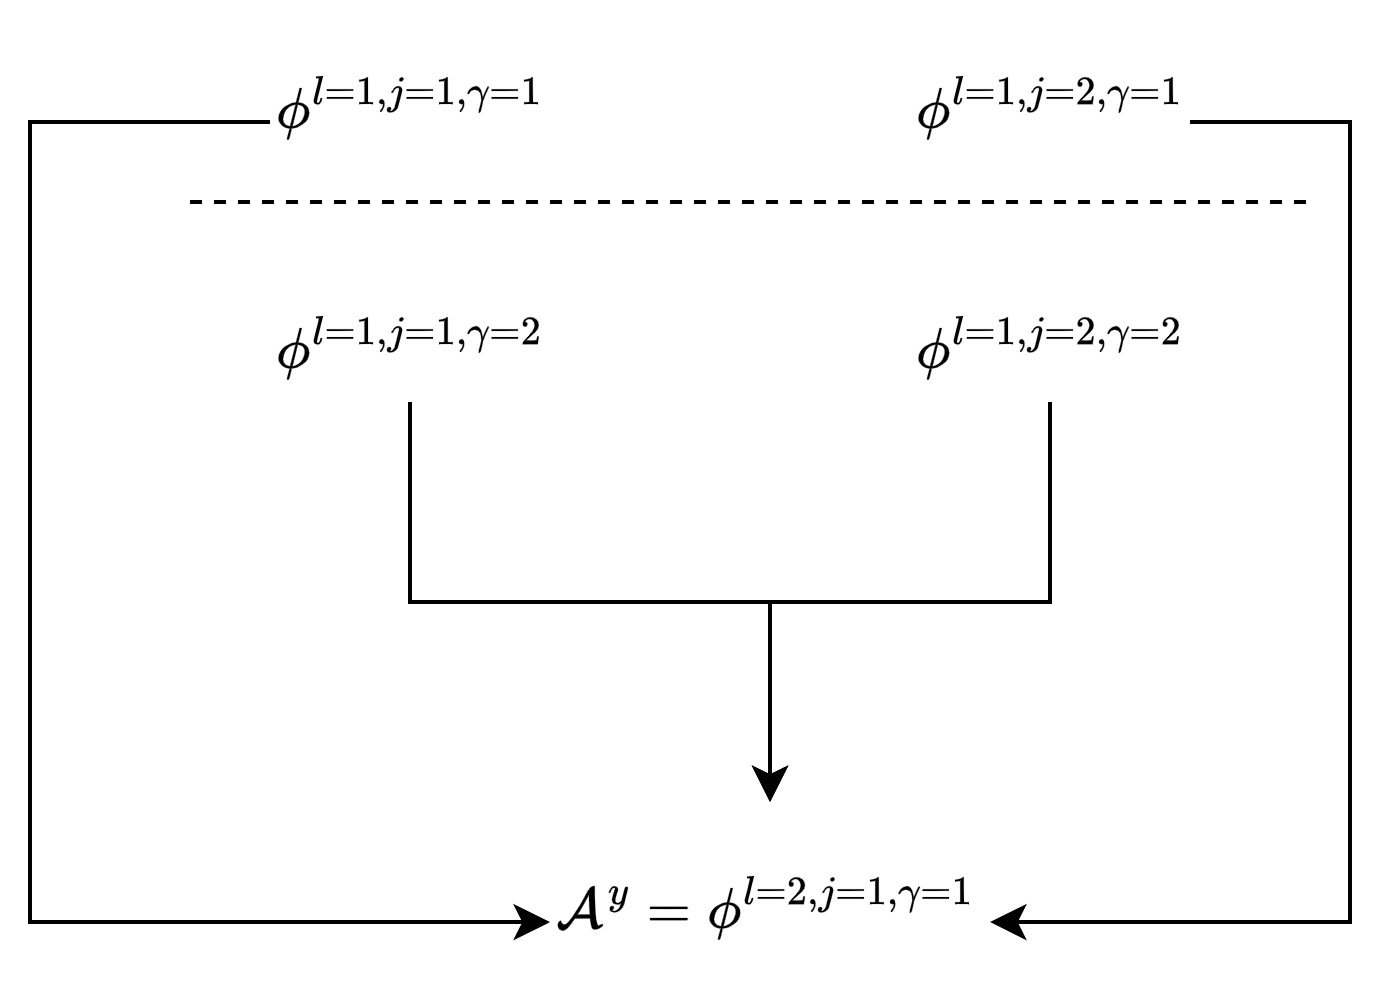
\includegraphics[width=0.9\linewidth]{matematicas/descomp_ht_rank_2_paso_2}
        \caption{Segundo paso. En la construcción del tensor $\mathcal{A}^y$ participan los cuatro tensores $\phi^{l=2, j, \gamma}$}
    \end{subfigure}
    \caption{Ejemplo gráfico del proceso de construcción del tensor $\mathcal{A}^y$ a través de la descomposición \textit{HT}. Hemos dividido el proceso de construcción en dos pasos. Ahora $r = 2$. Por lo tanto, en cada posición de cada capa, tenemos dos tensores. Seguimos teniendo $L = 2$ capas. }
    \label{img:diagrama_ht_complejo}
\end{figure}

\todo{Comentar en algún lado que $L = log_2(N)$. Además, estamos viendo en estos diagramas y en la ecuación principal \eqref{eq:descomposicion_ht} que estamos combinando dos a dos tensores, reduciendo en 2. Por eso es conveniente suponer que el orden de $\mathcal{A}^y$ es una potencia de dos}

\subsection{Parámetros del modelo} \label{msubs:parametros_modelo_ht}

Nuestro modelo viene dado por los siguientes parámetros:

\begin{itemize}
    \item Vectores iniciales:
        \begin{equation}
            \{\nv{\varphi^{j, \alpha}} \in \R^M: j \in \deltaset{N}, \alpha \in \deltaset{r_0}  \}
        \end{equation}

        Es decir, que aportan $M \cdot r_0 \cdot N$ coeficientes
    \item Pesos intermedios:

        \begin{equation}
            \{ a^{l, j, \gamma}_{\alpha} \in \R: l \in \deltaset{L-1}, j \in \deltaset{\frac{N}{2^l}}, \gamma \in \deltaset{r_l}, \alpha \in \deltaset{r_{l-1}} \}
        \end{equation}

        Por tanto, están aportando $\sum_{l = 1}^{L-1} r_{l-1} \cdot \frac{N}{2^l} \cdot r_l$ coeficientes.

    \item Pesos finales:

        \begin{equation}
            \{a^{L, y}_{\alpha}: y \in \deltaset{Y}, \alpha \in \deltaset{r_{L-1}} \}
        \end{equation}

        Por tanto, están aportando $r_{L-1} \cdot Y$ coeficientes.
\end{itemize}

Es decir, que nuestro modelo tiene

\begin{equation}
    M \cdot r_0 \cdot N + \sum_{l = 1}^{L-1} (r_{l-1} \cdot \frac{N}{2^l} \cdot r_l ) +
    r_{L-1} \cdot Y
\end{equation}

coeficientes. Si asumimos que todos los rangos son iguales, $r := r_0 = \ldots = r_{L-1}$, entonces el número de parámetros es:

\begin{equation}
\begin{split}
    M \cdot r \cdot N + \sum_{l = 1}^{L-1} r^2 \cdot \frac{N}{2^l} + r \cdot Y &= M \cdot r \cdot N + N \cdot r^2 \cdot \frac{2^{L-1} - 1}{2^{L-1}} + r \cdot Y \longmapsto \ldots \\
    \ldots & \encima{\longmapsto}{L \mapsto \infty} M \cdot r \cdot N + N \cdot r^2 + r \cdot Y
\end{split}
\end{equation}

donde hemos usado que:

\begin{equation}
    \sum_{l = 1}^{L-1} \frac{1}{2^l} = \frac{2^{L-1} - 1}{2^{L-1}}
\end{equation}

Podemos comprobar esto fácilmente:

\begin{proposicion}
    \begin{equation}
        \sum_{k = 1}^{N} \frac{1}{2^k} = \frac{2^N - 1}{2^N}; \dspace \forall N \in \N
    \end{equation}
\end{proposicion}

\begin{proof}
    Procederemos por inducción. Veamos que la ecuación se verifica para $N = 1$:

    \begin{equation}
        \sum_{k = 1}^{1} \frac{1}{2^k} = \frac{1}{2} = \frac{2^1 - 1}{2^1}
    \end{equation}

    Supuesto que la ecuación se cumple para $N$, veamos si la ecuación se cumple para $N + 1$:

    \begin{equation}
    \begin{split}
        \sum_{k = 1}^{N+1} \frac{1}{2^k} &= \sum_{k = 1}^{N} (\frac{1}{2^k}) + \frac{1}{2^{N+1}} \encima{=}{\text{hip. ind.}} \ldots \\
        \ldots &= \frac{2^N - 1}{2^N} + \frac{1}{2^{N+1}} = \ldots \\
        \ldots &= \frac{2^{N+1} - 2 + 1}{2^{N+1}} = \ldots \\
        \ldots &= \frac{2^{N+1} - 1}{2^{N+1}}
    \end{split}
    \end{equation}
\end{proof}
\todo{Tengo hecha esta demostración de forma directa en la página 49 de mis notas}

\todo{En el \textit{paper} esta ecuación la hacen igual a uno. Estoy bastante seguro de las cuentas pero no sé si me estoy confundiendo en algún detalle previo a plantear este paso}

\begin{proposicion}

    La descomposición \textit{HT} es universal. Es más, extiende la descomposición \textit{CP}. Esto es, cualquier tensor que pueda expresarse como la descomposición \textit{CP} con rango \textit{CP} $Z$, admite una descomposición \textit{HT} con rangos $r_1 = r_2 = \ldots = r_{L - 1} = Z$
\end{proposicion}

\begin{proof}

    \todo{En la página 8 del paper se da una indicación de cómo se hace esto}

\end{proof}

\begin{observacion}

    Aunque \textit{HT} sea una extensión de \textit{CP}, hay que tener en cuenta que el número de coeficientes crece.

    En el modelo \textit{CP} tenemos $N \cdot M \cdot Z + Z \cdot Y$ coeficientes que especificar (\customref{msubsec:parametros_modelo_cp}).

    En el modelo \textit{HT} tenemos $N \cdot M \cdot Z + N \cdot Z^2 \cdot \frac{2^{L-1} - 1}{2^{L-1}} + Z \cdot Y$, teniendo en cuenta que estamos considerando $r = Z$ (\customref{msubs:parametros_modelo_ht}).

    Por lo tanto, la diferencia en número de coeficientes viene dada por:

    \begin{equation}
        Z^2 \cdot \frac{2^{L-1} - 1}{2^{L-1}} \encima{\longmapsto}{L \mapsto \infty} N \cdot Z^2
    \end{equation}

    Por lo tanto, el número de parámetros crece de forma cuadrática. Sin embargo, como veremos más adelante, la ganancia en expresividad del modelo es exponencial.
    \todo{Revisitar esto cuando haya especificado formalmente qué significa ganancia exponencial en expresividad}

\end{observacion}

\subsection{Desarrollo del modelo}

El modelo \textit{HT} es el resultado de usar la descomposición \textit{HT} descrita en la ecuación \eqref{eq:descomposicion_ht} en nuestra función de puntuación \eqref{eq:puntuacion_general}. En esta sección, describiremos el modelo producido.

Como en el modelo \textit{CP}, el primer paso consiste en computar la capa de representación, $\{f_d(\nv{x_i}): d \in \deltaset{N}, i \in \deltaset{M}\}$. Esto genera $N \cdot M$ números reales, que serán transformados en las $L$ capas ocultas \eqref{eq:descomposicion_ht} que producen la salida.

Cada capa oculta se compone de una convolución $1 \times 1$ y un \textit{product pooling} con tamaño de ventana 2. En el modelo \textit{CP}, el \textit{product pooling} era global, colapsando las \textit{feature maps}. En este \textit{product pooling} reducimos el número de \textit{feature maps} a la mitad en cada paso.

Por lo tanto, tras las $L = log_2(N)$ capas ocultas, las $N$ \textit{feature maps} iniciales acaban siendo una sola. Por lo tanto, acabamos con una lista de $r_{L - 1}$ coeficientes sobre los que aplicamos una última capa oculta, dada por la última ecuación de \eqref{eq:descomposicion_ht}.

Nuestra red realiza \textit{product pooling} con un tamaño de ventana 2, sin \textit{overlapping} gracias al hecho de que estamos combinando los tensores dos a dos, de forma contigua, como indican \customref{img:diagrama_ht_simple} y \customref{img:diagrama_ht_complejo}. Como muestra \cite{matematicas:descomposicion_ht}, podríamos haber escogido otra forma de combinar los tensores. Por ejemplo, combinando más de dos en cada paso. Esto produciría diferentes combinaciones de tamaños de ventana en el \textit{product pooling} y, por tanto, distintas profundidades.

\todo{Escribir en algún lugar que $L = log_2(N)$}

\todo{Es muy mal nombre}

\todo{Revisar la escritura de este apartado, porque es muy importante en el \textit{TFG}}

\todo{Crear un diagrama para explicar este modelo}

\subsection{Compartición de coeficientes}

Al igual que ocurría en el modelo \textit{CP}, nuestras convoluciones $1 \times 1$ son dependientes de la localización. En la práctica, las convoluciones en los modelos convolucionales son independientes de la localización, lo que se conoce como \textbf{compartición de coeficientes}. En \customref{subs:comparticion_parametros_cp} ya hemos comentado por qué es necesaria esta compartición de parámetros.

En el modelo \textit{HT} es muy fácil imponer la compartición de coeficientes, teniendo en cuenta los comentarios que hemos hecho en \customref{sec:modelo_ht}. Consideremos la ecuación de la capa $l$:

\begin{equation}
    \phi^{l, j, \gamma} := \sum_{\alpha = 1}^{r_{l-1}} a_{\alpha}^{l, j, \gamma} \cdot \phi^{l-1, 2j-1, \alpha} \otimes \phi^{l-1, 2j, \alpha}
\end{equation}

En $\phi^{l, j, \gamma}$:

\begin{itemize}
    \item $l$ indica la capa en la que nos encontramos
    \item $j$ indica la posición del tensor en la capa $l$
    \item $\gamma$ indica con qué tensor trabajamos en la posición $j$, porque podemos tener más de un tensor en cada posición (cuando $r_l > 1$)
\end{itemize}

Por lo tanto, los coeficientes $\nv{a^{l, j, \gamma}} := (a^{l, j, \gamma}_1, \ldots, a^{l, j, \gamma}_{r_{l-1}})$ no deberían depender de la posición $j$, es decir:

\begin{equation}
    \nv{a^{l, 1, \gamma}} = \nv{a^{l, 2, \gamma}} = \ldots = \nv{a^{l, N/2^l, \gamma}} =: \nv{a^{l, \gamma}}; \dspace \forall l \in \doubledeltaset{0}{L - 1} \dspace \forall \gamma \in \deltaset{r_l}
\end{equation}

Como ocurría en \customref{subs:comparticion_parametros_cp}, la compartición de parámetros provoca que nuestro modelo pierda la universalidad. Esto es, nuestro modelo no puede representar cualquier tensor, independientemente de los valores de $L$ o $r_l$. Aunque en este caso, los tensores que podemos generar con la compartición de parámetros no están limitados a ser simétricos, como en el caso \textit{CP}. Esto ya es un primer indicativo de que el modelo \textit{HT} es más expresivo que el modelo \textit{CP}.
